\section{1. Leitungscodes}
\paragraph{Aufgabe 1.1:}
	Kodieren Sie den angegebene Bitsequenz mittels normalem Manchester-Code und geben Sie die resultierenden Signalfolge an.

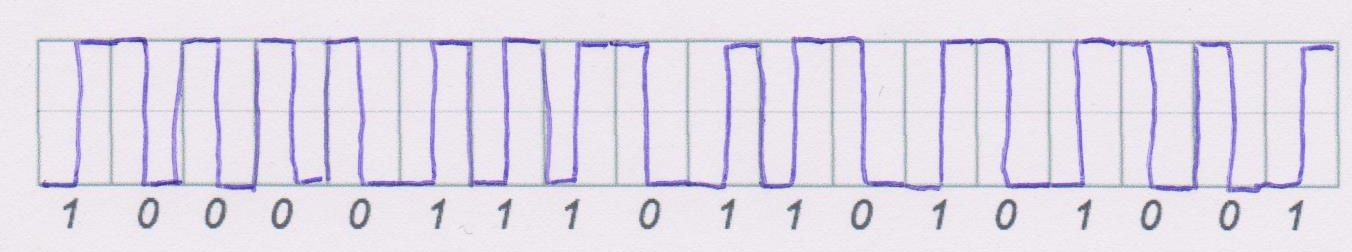
\includegraphics[scale=0.2]{blatt3_1_1}
\paragraph{Aufgabe 1.2:}
	Kodieren Sie den angegebene Bitsequenz mittels differentiellem Manchester-Code und geben Sie die resultierenden Signalfolge an. Gibt es eine eindeutige Lösung ?
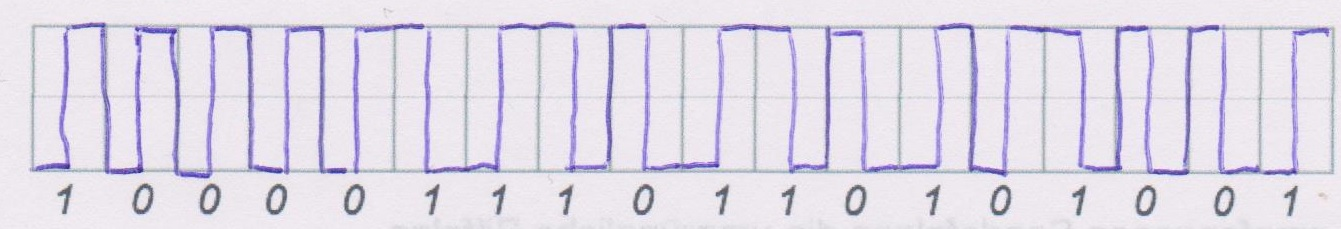
\includegraphics[scale=0.2]{blatt3_1_2}

\paragraph{Aufgabe 1.3:}
	Diskutieren und vergleichen (Tip: Rauschen) Sie kurz die Eigenschaften der beiden Leitungscodes.
\paragraph{Antwort:}
    Der differentielle Manchestercode hat im Vergleich zum Normalen das Problem,
    dass ein Rauschen zum Bitanfang falsche Symbole einstreuen kann. Da beim
    normalen Manchestercode eine Flanke wichtig ist, die an mehreren Stellen
    während des Bits abgetastet und damit in überprüft werden kann, würde ein
    eingestreuter Polaritätswechsel am Anfang  ein falsches Bit darstellen und
    die Synchronisation durcheinanderbringen, wenn der Wechsel lange genug
    anhält um einen Flankenwechsel in der Bitmitte zu erzeugen.
    
    Der Aufbau des Differentiellen lässt sich leichter logisch trennen, da der
    Flankenwechsel in der Bitmitte garantiert ist und nichts mit dem zu
    übertragenden Bit zu tun hat. Daher kann man eine Einheit des Empfängers auf
    den Flankenwechsel achten lassen und damit den Takt regenerieren lassen und
    eine andere Einheit auf das zu übertragende Bit. Außerdem ist die
    Taktrückgewinnung und der Bitempfang zeitlich voneinander getrennt. Der
    normale Manchestercode ist hierbei verzahnter, da ein Polaritätwechsel zu 
    Anfang nur im Falle mehrere gleicher Bits passiert.

\section{2. Codemultiplex}
Gegeben seien die Walsh-Hadamard-Sequenzen der Länge 8 aus dem Skript.\\
Zu senden sind an den Empfänger 7 die Bitfolge $110$ und an den Empfänger 3 die Bitfolge $101$.
\paragraph{Aufgabe 1.1:}
	Berechnen Sie die zu sendenden Sendefolgen.
\paragraph{Antwort:} Die zu sendende Bitfolge ergibt sich aus der Addition beider Bitfolgen
	\begin{enumerate}

	\item Die Bitfolge für Empfänger $3$
	
		\begin{tabular}{|c||c|c|c|c|c|c|c|c|}
		\hline 1: & -1 & -1 & +1 & +1 & -1 & -1 & +1 & +1 \\ 
		\hline 0: & +1 & +1 & -1 & -1 & +1 & +1 & -1 & -1 \\ 
		\hline 1: & -1 & -1 & +1 & +1 & -1 & -1 & +1 & +1 \\ 
		\hline 
		\end{tabular} 
	
	\item Die Bitfolge für Empfänger $7$
		
		\begin{tabular}{|c||c|c|c|c|c|c|c|c|}
		\hline 1: & -1 & -1 & +1 & +1 & +1 & +1 & -1 & -1 \\ 
		\hline 1: & -1 & -1 & +1 & +1 & +1 & +1 & -1 & -1 \\ 
		\hline 0: & +1 & +1 & -1 & -1 & -1 & -1 & +1 & +1 \\ 
		\hline 
		\end{tabular} 
		
	\item Die Addierte Bitfolge ist demnach
	
		\begin{tabular}{|c|c|c|c|c|c|c|c|}
		\hline -1-1 & -1-1 & +1+1 & +1+1 & -1+1 & -1+1 & +1-1 & +1-1 \\
		$\Downarrow$ & $\Downarrow$ & $\Downarrow$ & $\Downarrow$ & $\Downarrow$ & $\Downarrow$ & $\Downarrow$ & $\Downarrow$ \\
		-2 & -2 & +2 & +2 & 0 & 0 & 0 & 0 \\ 
		\hline +1-1 & +1-1 & -1+1 & -1+1 & +1+1 & +1+1 & -1-1 & -1-1 \\
		$\Downarrow$ & $\Downarrow$ & $\Downarrow$ & $\Downarrow$ & $\Downarrow$ & $\Downarrow$ & $\Downarrow$ & $\Downarrow$ \\
		0 & 0 & 0 & 0 & +2 & +2 & -2 & -2 \\ 
		\hline -1+1 & -1+1 & +1-1 & +1-1 & -1-1 & -1-1 & +1+1 & +1+1 \\ 
		$\Downarrow$ & $\Downarrow$ & $\Downarrow$ & $\Downarrow$ & $\Downarrow$ & $\Downarrow$ & $\Downarrow$ & $\Downarrow$ \\
		0 & 0 & 0 & 0 & -2 & -2 & 2 & 2 \\
		\hline 
		\end{tabular} 
	
	\end{enumerate}
\paragraph{Aufgabe 1.2:}
	Berechnen Sie aus den empfangenen Sendefolgen die ursprüngliche Bitfolge.
\paragraph{Antwort:} Um die gesendeten Sendefolgen zu entschlüsseln müssen wir jetzt einfach das Skalarprodukt aus empfangener Folge und eigenem Schlüssel bilden.
	\begin{enumerate}
		\item Empfänger $3$
		
			\begin{tabular}{|c|c|c|c|c|c|c|c|c|c|}
			\hline empfangene Folge & -2 & -2 & 2 & 2 & 0 & 0 & 0 & 0 &  \\ 
			$\times$ eigener Schlüssel & 1 & 1 & -1 & -1 & 1 & 1 & -1 & -1 &  \\ 
			= & -2 & -2 & -2 & -2 & 0 & 0 & 0 & 0 & $\sum = -8 \Rightarrow \text{gesendetes Bit: 1}$ \\ 
			\hline empfangene Folge & 0 & 0 & 0 & 0 & 2 & 2 & -2 & -2 &  \\ 
			$\times$ eigener Schlüssel & 1 & 1 & -1 & -1 & 1 & 1 & -1 & -1 &  \\ 
			= & 0 & 0 & 0 & 0 & 2 & 2 & 2 & 2 & $\sum = 8 \Rightarrow \text{gesendetes Bit: 0}$ \\ 
			\hline empfangene Folge & 0 & 0 & 0 & 0 & -2 & -2 & 2 & 2 &  \\ 
			$\times$ eigener Schlüssel & 1 & 1 & -1 & -1 & 1 & 1 & -1 & -1 &  \\ 
			= & 0 & 0 & 0 & 0 & -2 & -2 & -2 & -2 & $\sum = -8 \Rightarrow \text{gesendetes Bit: 1}$ \\ 
			\hline 
			\end{tabular} 
		
		\item Empfänger $7$	
		
			\begin{tabular}{|c|c|c|c|c|c|c|c|c|c|}
			\hline empfangene Folge & -2 & -2 & 2 & 2 & 0 & 0 & 0 & 0 &  \\ 
			$\times$ eigener Schlüssel & 1 & 1 & -1 & -1 & -1 & -1 & 1 & 1 &  \\ 
			= & -2 & -2 & -2 & -2 & 0 & 0 & 0 & 0 & $\sum = -8 \Rightarrow \text{gesendetes Bit: 1}$ \\ 
			\hline empfangene Folge & 0 & 0 & 0 & 0 & 2 & 2 & -2 & -2 &  \\ 
			$\times$ eigener Schlüssel & 1 & 1 & -1 & -1 & -1 & -1 & 1 & 1 &  \\ 
			= & 0 & 0 & 0 & 0 & -2 & -2 & -2 & -2 & $\sum = -8 \Rightarrow \text{gesendetes Bit: 1}$ \\ 
			\hline empfangene Folge & 0 & 0 & 0 & 0 & -2 & -2 & 2 & 2 &  \\
			$\times$ eigener Schlüssel & 1 & 1 & -1 & -1 & -1 & -1 & 1 & 1 &  \\ 
			= & 0 & 0 & 0 & 0 & 2 & 2 & 2 & 2 & $\sum = 8 \Rightarrow \text{gesendetes Bit: 0}$ \\ 
			\hline 
			\end{tabular} 
		
	\end{enumerate}